\documentclass[11pt,a4paper]{report}
\usepackage[T1]{fontenc}
\usepackage{graphicx}
\usepackage{isabelle,isabellesym}
\usepackage{pdfsetup}

\urlstyle{rm}
\isabellestyle{it}

\begin{document}

\title{Hoare Logic for Parallel Programs}
\author{Leonor Prensa Nieto}
\maketitle

\begin{abstract}\noindent
  In the following theories a formalization of the Owicki-Gries and
  the rely-guarantee methods is presented. These methods are widely
  used for correctness proofs of parallel imperative programs with
  shared variables.  We define syntax, semantics and proof rules in
  Isabelle/HOL.  The proof rules also provide for programs
  parameterized in the number of parallel components. Their
  correctness w.r.t.\ the semantics is proven.  Completeness proofs
  for both methods are extended to the new case of parameterized
  programs. (These proofs have not been formalized in Isabelle. They
  can be found in~\cite{Prensa-PhD}.)  Using this formalizations we
  verify several non-trivial examples for parameterized and
  non-parameterized programs.  For the automatic generation of
  verification conditions with the Owicki-Gries method we define a
  tactic based on the proof rules.  The most involved examples are the
  verification of two garbage-collection algorithms, the second one
  parameterized in the number of mutators.

For excellent descriptions of this work see
\cite{NipkowP-FASE99,PrenEsp00,Prensa-PhD,Prensa-ESOP03}.

\end{abstract}

\pagestyle{plain}
\thispagestyle{empty}
\tableofcontents

\clearpage

\begin{center}
  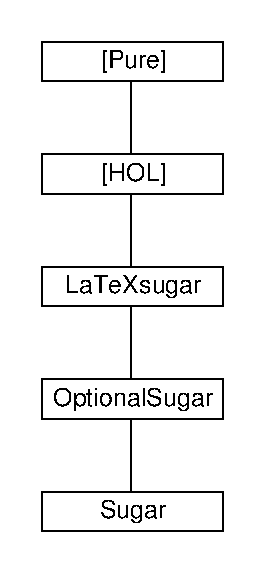
\includegraphics[scale=0.7]{session_graph}  
\end{center}

\newpage

\parindent 0pt\parskip 0.5ex
%
\begin{isabellebody}%
\def\isabellecontext{Locales}%
%
\isadelimtheory
\isanewline
%
\endisadelimtheory
%
\isatagtheory
%
\endisatagtheory
{\isafoldtheory}%
%
\isadelimtheory
%
\endisadelimtheory
%
\isadelimML
%
\endisadelimML
%
\isatagML
%
\endisatagML
{\isafoldML}%
%
\isadelimML
%
\endisadelimML
%
\isamarkupsection{Overview%
}
\isamarkuptrue%
%
\begin{isamarkuptext}%
The present text is based on~\cite{Ballarin2004a}.  It was updated
  for for Isabelle2005, but does not cover locale interpretation.

  Locales are an extension of the Isabelle proof assistant.  They
  provide support for modular reasoning. Locales were initially
  developed by Kamm\"uller~\cite{Kammuller2000} to support reasoning
  in abstract algebra, but are applied also in other domains --- for
  example, bytecode verification~\cite{Klein2003}.

  Kamm\"uller's original design, implemented in Isabelle99, provides, in
  addition to
  means for declaring locales, a set of ML functions that were used
  along with ML tactics in a proof.  In the meantime, the input format
  for proof in Isabelle has changed and users write proof
  scripts in ML only rarely if at all.  Two new proof styles are
  available, and can
  be used interchangeably: linear proof scripts that closely resemble ML
  tactics, and the structured Isar proof language by
  Wenzel~\cite{Wenzel2002a}.  Subsequently, Wenzel re-implemented
  locales for
  the new proof format.  The implementation, available with
  Isabelle2003, constitutes a complete re-design and exploits that
  both Isar and locales are based on the notion of context,
  and thus locales are seen as a natural extension of Isar.
  Nevertheless, locales can also be used with proof scripts:
  their use does not require a deep understanding of the structured
  Isar proof style.

  At the same time, Wenzel considerably extended locales.  The most
  important addition are locale expressions, which allow to combine
  locales more freely.  Previously only
  linear inheritance was possible.  Now locales support multiple
  inheritance through a normalisation algorithm.  New are also
  structures, which provide special syntax for locale parameters that
  represent algebraic structures.

  Unfortunately, Wenzel provided only an implementation but hardly any
  documentation.  Besides providing documentation, the present paper
  is a high-level description of locales, and in particular locale
  expressions.  It is meant as a first step towards the semantics of
  locales, and also as a base for comparing locales with module concepts
  in other provers.  It also constitutes the base for future
  extensions of locales in Isabelle.
  The description was derived mainly by experimenting
  with locales and partially also by inspecting the code.

  The main contribution of the author of the present paper is the
  abstract description of Wenzel's version of locales, and in
  particular of the normalisation algorithm for locale expressions (see
  Section~\ref{sec-normal-forms}).  Contributions to the
  implementation are confined to bug fixes and to provisions that
  enable the use of locales with linear proof scripts.

  Concepts are introduced along with examples, so that the text can be
  used as tutorial.  It is assumed that the reader is somewhat
  familiar with Isabelle proof scripts.  Examples have been phrased as
  structured
  Isar proofs.  However, in order to understand the key concepts,
  including locales expressions and their normalisation, detailed
  knowledge of Isabelle is not necessary. 

\nocite{Nipkow2003,Wenzel2002b,Wenzel2003}%
\end{isamarkuptext}%
\isamarkuptrue%
%
\isamarkupsection{Locales: Beyond Proof Contexts%
}
\isamarkuptrue%
%
\begin{isamarkuptext}%
In tactic-based provers the application of a sequence of proof
  tactics leads to a proof state.  This state is usually hard to
  predict from looking at the tactic script, unless one replays the
  proof step-by-step.  The structured proof language Isar is
  different.  It is additionally based on \emph{proof contexts},
  which are directly visible in Isar scripts, and since tactic
  sequences tend to be short, this commonly leads to clearer proof
  scripts.

  Goals are stated with the \textbf{theorem}
  command.  This is followed by a proof.  When discharging a goal
  requires an elaborate argument
  (rather than the application of a single tactic) a new context
  may be entered (\textbf{proof}).  Inside the context, variables may
  be fixed (\textbf{fix}), assumptions made (\textbf{assume}) and
  intermediate goals stated (\textbf{have}) and proved.  The
  assumptions must be dischargeable by premises of the surrounding
  goal, and once this goal has been proved (\textbf{show}) the proof context
  can be closed (\textbf{qed}). Contexts inherit from surrounding
  contexts, but it is not possible
  to export from them (with exception of the proved goal);
  they ``disappear'' after the closing \textbf{qed}.
  Facts may have attributes --- for example, identifying them as
  default to the simplifier or classical reasoner.

  Locales extend proof contexts in various ways:
  \begin{itemize}
  \item
    Locales are usually \emph{named}.  This makes them persistent.
  \item
    Fixed variables may have \emph{syntax}.
  \item
    It is possible to \emph{add} and \emph{export} facts.
  \item
    Locales can be combined and modified with \emph{locale
    expressions}.
  \end{itemize}
  The Locales facility extends the Isar language: it provides new ways
  of stating and managing facts, but it does not modify the language
  for proofs.  Its purpose is to support writing modular proofs.%
\end{isamarkuptext}%
\isamarkuptrue%
%
\isamarkupsection{Simple Locales%
}
\isamarkuptrue%
%
\isamarkupsubsection{Syntax and Terminology%
}
\isamarkuptrue%
%
\begin{isamarkuptext}%
The grammar of Isar is extended by commands for locales as shown in
  Figure~\ref{fig-grammar}.
  A key concept, introduced by Wenzel, is that
  locales are (internally) lists
  of \emph{context elements}.  There are five kinds, identified
  by the keywords \textbf{fixes}, \textbf{constrains},
  \textbf{assumes}, \textbf{defines} and \textbf{notes}.

  \begin{figure}
  \hrule
  \vspace{2ex}
  \begin{small}
  \begin{tabular}{l>$c<$l}
  \textit{attr-name} & ::=
  & \textit{name} $|$ \textit{attribute} $|$
    \textit{name} \textit{attribute} \\

  \textit{locale-expr}  & ::= 
  & \textit{locale-expr1} ( ``\textbf{+}'' \textit{locale-expr1} )$^*$ \\
  \textit{locale-expr1} & ::=
  & ( \textit{qualified-name} $|$
    ``\textbf{(}'' \textit{locale-expr} ``\textbf{)}'' ) \\
  & & ( \textit{name} [ \textit{mixfix} ] $|$ ``\textbf{\_}'' )$^*$ \\

  \textit{fixes} & ::=
  & \textit{name} [ ``\textbf{::}'' \textit{type} ]
    [ ``\textbf{(}'' \textbf{structure} ``\textbf{)}'' $|$
    \textit{mixfix} ] \\
  \textit{constrains} & ::=
  & \textit{name} ``\textbf{::}'' \textit{type} \\
  \textit{assumes} & ::=
  & [ \textit{attr-name} ``\textbf{:}'' ] \textit{proposition} \\
  \textit{defines} & ::=
  & [ \textit{attr-name} ``\textbf{:}'' ] \textit{proposition} \\
  \textit{notes} & ::=
  & [ \textit{attr-name} ``\textbf{=}'' ]
    ( \textit{qualified-name} [ \textit{attribute} ] )$^+$ \\

  \textit{element} & ::=
  & \textbf{fixes} \textit{fixes} ( \textbf{and} \textit{fixes} )$^*$ \\
  & |
  & \textbf{constrains} \textit{constrains}
    ( \textbf{and} \textit{constrains} )$^*$ \\
  & |
  & \textbf{assumes} \textit{assumes} ( \textbf{and} \textit{assumes} )$^*$ \\
  & |
  & \textbf{defines} \textit{defines} ( \textbf{and} \textit{defines} )$^*$ \\
  & |
  & \textbf{notes} \textit{notes} ( \textbf{and} \textit{notes} )$^*$ \\
  \textit{element1} & ::=
  & \textit{element} \\
  & | & \textbf{includes} \textit{locale-expr} \\

  \textit{locale} & ::=
  & \textit{element}$^+$ \\
  & | & \textit{locale-expr} [ ``\textbf{+}'' \textit{element}$^+$ ] \\

  \textit{in-target} & ::=
  & ``\textbf{(}'' \textbf{in} \textit{qualified-name} ``\textbf{)}'' \\

  \textit{theorem} & ::= & ( \textbf{theorem} $|$ \textbf{lemma} $|$
    \textbf{corollary} ) [ \textit{in-target} ] [ \textit{attr-name} ] \\

  \textit{theory-level} & ::= & \ldots \\
  & | & \textbf{locale} \textit{name} [ ``\textbf{=}''
    \textit{locale} ] \\
  % note: legacy "locale (open)" omitted.
  & | & ( \textbf{theorems} $|$ \textbf{lemmas} ) \\
  & & [ \textit{in-target} ] [ \textit{attr-name} ``\textbf{=}'' ]
    ( \textit{qualified-name} [ \textit{attribute} ] )$^+$ \\
  & | & \textbf{declare} [ \textit{in-target} ] ( \textit{qualified-name}
    [ \textit{attribute} ] )$^+$ \\
  & | & \textit{theorem} \textit{proposition} \textit{proof} \\
  & | & \textit{theorem} \textit{element1}$^*$
    \textbf{shows} \textit{proposition} \textit{proof} \\
  & | & \textbf{print\_locale} \textit{locale} \\
  & | & \textbf{print\_locales}
  \end{tabular}
  \end{small}
  \vspace{2ex}
  \hrule
  \caption{Locales extend the grammar of Isar.}
  \label{fig-grammar}
  \end{figure}

  At the theory level --- that is, at the outer syntactic level of an
  Isabelle input file --- \textbf{locale} declares a named
  locale.  Other kinds of locales,
  locale expressions and unnamed locales, will be introduced later.  When
  declaring a named locale, it is possible to \emph{import} another
  named locale, or indeed several ones by importing a locale
  expression.  The second part of the declaration, also optional,
  consists of a number of context element declarations.

  A number of Isar commands have an additional, optional \emph{target}
  argument, which always refers to a named locale.  These commands
  are \textbf{theorem} (together with \textbf{lemma} and
  \textbf{corollary}),  \textbf{theorems} (and
  \textbf{lemmas}), and \textbf{declare}.  The effect of specifying a target is
  that these commands focus on the specified locale, not the
  surrounding theory.  Commands that are used to
  prove new theorems will add them not to the theory, but to the
  locale.  Similarly, \textbf{declare} modifies attributes of theorems
  that belong to the specified target.  Additionally, for
  \textbf{theorem} (and related commands), theorems stored in the target
  can be used in the associated proof scripts.

  The Locales package provides a \emph{long goals format} for
  propositions stated with \textbf{theorem} (and friends).  While
  normally a goal is just a formula, a long goal is a list of context
  elements, followed by the keyword \textbf{shows}, followed by the
  formula.  Roughly speaking, the context elements are
  (additional) premises.  For an example, see
  Section~\ref{sec-includes}.  The list of context elements in a long goal
  is also called \emph{unnamed locale}.

  Finally, there are two commands to inspect locales when working in
  interactive mode: \textbf{print\_locales} prints the names of all
  targets
  visible in the current theory, \textbf{print\_locale} outputs the
  elements of a named locale or locale expression.

  The following presentation will use notation of
  Isabelle's meta logic, hence a few sentences to explain this.
  The logical
  primitives are universal quantification (\isa{{\isasymAnd}}), entailment
  (\isa{{\isasymLongrightarrow}}) and equality (\isa{{\isasymequiv}}).  Variables (not bound
  variables) are sometimes preceded by a question mark.  The logic is
  typed.  Type variables are denoted by \isa{{\isacharprime}a}, \isa{{\isacharprime}b}
  etc., and \isa{{\isasymRightarrow}} is the function type.  Double brackets \isa{{\isasymlbrakk}} and \isa{{\isasymrbrakk}} are used to abbreviate nested entailment.%
\end{isamarkuptext}%
\isamarkuptrue%
%
\isamarkupsubsection{Parameters, Assumptions and Facts%
}
\isamarkuptrue%
%
\begin{isamarkuptext}%
From a logical point of view a \emph{context} is a formula schema of
  the form
\[
  \isa{{\isasymAnd}x\isactrlsub {\isadigit{1}}{\isasymdots}x\isactrlsub n{\isachardot}\ {\isasymlbrakk}\ C\isactrlsub {\isadigit{1}}{\isacharsemicolon}\ {\isasymdots}\ {\isacharsemicolon}C\isactrlsub m\ {\isasymrbrakk}\ {\isasymLongrightarrow}\ {\isasymdots}}
\]
  The variables $\isa{x\isactrlsub {\isadigit{1}}}, \ldots, \isa{x\isactrlsub n}$ are
  called \emph{parameters}, the premises $\isa{C\isactrlsub {\isadigit{1}}}, \ldots,
  \isa{C\isactrlsub n}$ \emph{assumptions}.  A formula \isa{F}
  holds in this context if
\begin{equation}
\label{eq-fact-in-context}
  \isa{{\isasymAnd}x\isactrlsub {\isadigit{1}}{\isasymdots}x\isactrlsub n{\isachardot}\ {\isasymlbrakk}\ C\isactrlsub {\isadigit{1}}{\isacharsemicolon}\ {\isasymdots}\ {\isacharsemicolon}C\isactrlsub m\ {\isasymrbrakk}\ {\isasymLongrightarrow}\ F}
\end{equation}
  is valid.  The formula is called a \emph{fact} of the context.

  A locale allows fixing the parameters \isa{x\isactrlsub {\isadigit{1}}{\isacharcomma}\ {\isasymdots}{\isacharcomma}\ x\isactrlsub n} and making the assumptions \isa{C\isactrlsub {\isadigit{1}}{\isacharcomma}\ {\isasymdots}{\isacharcomma}\ C\isactrlsub m}.  This implicitly builds the context in
  which the formula \isa{F} can be established.
  Parameters of a locale correspond to the context element
  \textbf{fixes}, and assumptions may be declared with
  \textbf{assumes}.  Using these context elements one can define
  the specification of semigroups.%
\end{isamarkuptext}%
\isamarkuptrue%
\isacommand{locale}\isamarkupfalse%
\ semi\ {\isacharequal}\isanewline
\ \ \isakeyword{fixes}\ prod\ {\isacharcolon}{\isacharcolon}\ {\isachardoublequoteopen}{\isacharbrackleft}{\isacharprime}a{\isacharcomma}\ {\isacharprime}a{\isacharbrackright}\ {\isasymRightarrow}\ {\isacharprime}a{\isachardoublequoteclose}\ {\isacharparenleft}\isakeyword{infixl}\ {\isachardoublequoteopen}{\isasymcdot}{\isachardoublequoteclose}\ {\isadigit{7}}{\isadigit{0}}{\isacharparenright}\isanewline
\ \ \isakeyword{assumes}\ assoc{\isacharcolon}\ {\isachardoublequoteopen}{\isacharparenleft}x\ {\isasymcdot}\ y{\isacharparenright}\ {\isasymcdot}\ z\ {\isacharequal}\ x\ {\isasymcdot}\ {\isacharparenleft}y\ {\isasymcdot}\ z{\isacharparenright}{\isachardoublequoteclose}%
\begin{isamarkuptext}%
The parameter \isa{prod} has a
  syntax annotation enabling the infix ``\isa{{\isasymcdot}}'' in the
  assumption of associativity.  Parameters may have arbitrary mixfix
  syntax, like constants.  In the example, the type of \isa{prod} is
  specified explicitly.  This is not necessary.  If no type is
  specified, a most general type is inferred simultaneously for all
  parameters, taking into account all assumptions (and type
  specifications of parameters, if present).%
\footnote{Type inference also takes into account type constraints,
  definitions and import, as introduced later.}

  Free variables in assumptions are implicitly universally quantified,
  unless they are parameters.  Hence the context defined by the locale
  \isa{semi} is
\[
  \isa{{\isasymAnd}prod{\isachardot}\ {\isasymlbrakk}\ {\isasymAnd}x\ y\ z{\isachardot}\ prod\ {\isacharparenleft}prod\ x\ y{\isacharparenright}\ z\ {\isacharequal}\ prod\ x\ {\isacharparenleft}prod\ y\ z{\isacharparenright}\ {\isasymrbrakk}\ {\isasymLongrightarrow}\ {\isasymdots}}
\]
  The locale can be extended to commutative semigroups.%
\end{isamarkuptext}%
\isamarkuptrue%
\isacommand{locale}\isamarkupfalse%
\ comm{\isacharunderscore}semi\ {\isacharequal}\ semi\ {\isacharplus}\isanewline
\ \ \isakeyword{assumes}\ comm{\isacharcolon}\ {\isachardoublequoteopen}x\ {\isasymcdot}\ y\ {\isacharequal}\ y\ {\isasymcdot}\ x{\isachardoublequoteclose}%
\begin{isamarkuptext}%
This locale \emph{imports} all elements of \isa{semi}.  The
  latter locale is called the import of \isa{comm{\isacharunderscore}semi}. The
  definition adds commutativity, hence its context is
\begin{align*%
}
  \isa{{\isasymAnd}prod{\isachardot}\ {\isasymlbrakk}} & 
  \isa{{\isasymAnd}x\ y\ z{\isachardot}\ prod\ {\isacharparenleft}prod\ x\ y{\isacharparenright}\ z\ {\isacharequal}\ prod\ x\ {\isacharparenleft}prod\ y\ z{\isacharparenright}{\isacharsemicolon}} \\
  & \isa{{\isasymAnd}x\ y{\isachardot}\ prod\ x\ y\ {\isacharequal}\ prod\ y\ x\ {\isasymrbrakk}\ {\isasymLongrightarrow}\ {\isasymdots}}
\end{align*%
}
  One may now derive facts --- for example, left-commutativity --- in
  the context of \isa{comm{\isacharunderscore}semi} by specifying this locale as
  target, and by referring to the names of the assumptions \isa{assoc} and \isa{comm} in the proof.%
\end{isamarkuptext}%
\isamarkuptrue%
\isacommand{theorem}\isamarkupfalse%
\ {\isacharparenleft}\isakeyword{in}\ comm{\isacharunderscore}semi{\isacharparenright}\ lcomm{\isacharcolon}\isanewline
\ \ {\isachardoublequoteopen}x\ {\isasymcdot}\ {\isacharparenleft}y\ {\isasymcdot}\ z{\isacharparenright}\ {\isacharequal}\ y\ {\isasymcdot}\ {\isacharparenleft}x\ {\isasymcdot}\ z{\isacharparenright}{\isachardoublequoteclose}\isanewline
%
\isadelimproof
%
\endisadelimproof
%
\isatagproof
\isacommand{proof}\isamarkupfalse%
\ {\isacharminus}\isanewline
\ \ \isacommand{have}\isamarkupfalse%
\ {\isachardoublequoteopen}x\ {\isasymcdot}\ {\isacharparenleft}y\ {\isasymcdot}\ z{\isacharparenright}\ {\isacharequal}\ {\isacharparenleft}x\ {\isasymcdot}\ y{\isacharparenright}\ {\isasymcdot}\ z{\isachardoublequoteclose}\ \isacommand{by}\isamarkupfalse%
\ {\isacharparenleft}simp\ add{\isacharcolon}\ assoc{\isacharparenright}\isanewline
\ \ \isacommand{also}\isamarkupfalse%
\ \isacommand{have}\isamarkupfalse%
\ {\isachardoublequoteopen}{\isasymdots}\ {\isacharequal}\ {\isacharparenleft}y\ {\isasymcdot}\ x{\isacharparenright}\ {\isasymcdot}\ z{\isachardoublequoteclose}\ \isacommand{by}\isamarkupfalse%
\ {\isacharparenleft}simp\ add{\isacharcolon}\ comm{\isacharparenright}\isanewline
\ \ \isacommand{also}\isamarkupfalse%
\ \isacommand{have}\isamarkupfalse%
\ {\isachardoublequoteopen}{\isasymdots}\ {\isacharequal}\ y\ {\isasymcdot}\ {\isacharparenleft}x\ {\isasymcdot}\ z{\isacharparenright}{\isachardoublequoteclose}\ \isacommand{by}\isamarkupfalse%
\ {\isacharparenleft}simp\ add{\isacharcolon}\ assoc{\isacharparenright}\isanewline
\ \ \isacommand{finally}\isamarkupfalse%
\ \isacommand{show}\isamarkupfalse%
\ {\isacharquery}thesis\ \isacommand{{\isachardot}}\isamarkupfalse%
\isanewline
\isacommand{qed}\isamarkupfalse%
%
\endisatagproof
{\isafoldproof}%
%
\isadelimproof
%
\endisadelimproof
%
\begin{isamarkuptext}%
In this equational Isar proof, ``\isa{{\isasymdots}}'' refers to the
  right hand side of the preceding equation.
  After the proof is finished, the fact \isa{lcomm} is added to
  the locale \isa{comm{\isacharunderscore}semi}.  This is done by adding a
  \textbf{notes} element to the internal representation of the locale,
  as explained the next section.%
\end{isamarkuptext}%
\isamarkuptrue%
%
\isamarkupsubsection{Locale Predicates and the Internal Representation of
  Locales%
}
\isamarkuptrue%
%
\begin{isamarkuptext}%
\label{sec-locale-predicates}
  In mathematical texts, often arbitrary but fixed objects with
  certain properties are considered --- for instance, an arbitrary but
  fixed group $G$ --- with the purpose of establishing facts valid for
  any group.  These facts are subsequently used on other objects that
  also have these properties.

  Locales permit the same style of reasoning.  Exporting a fact $F$
  generalises the fixed parameters and leads to a (valid) formula of the
  form of equation~(\ref{eq-fact-in-context}).  If a locale has many
  assumptions
  (possibly accumulated through a number of imports) this formula can
  become large and cumbersome.  Therefore, Wenzel introduced 
  predicates that abbreviate the assumptions of locales.  These
  predicates are not confined to the locale but are visible in the
  surrounding theory.

  The definition of the locale \isa{semi} generates the \emph{locale
  predicate} \isa{semi} over the type of the parameter \isa{prod},
  hence the predicate's type is \isa{{\isacharparenleft}{\isacharbrackleft}{\isacharprime}a{\isacharcomma}\ {\isacharprime}a{\isacharbrackright}\ {\isasymRightarrow}\ {\isacharprime}a{\isacharparenright}\ {\isasymRightarrow}\ bool}.  Its
  definition is
\begin{equation}
  \tag*{\isa{semi{\isacharunderscore}def}:} \isa{semi\ {\isacharquery}prod\ {\isasymequiv}\ {\isasymforall}x\ y\ z{\isachardot}\ {\isacharquery}prod\ {\isacharparenleft}{\isacharquery}prod\ x\ y{\isacharparenright}\ z\ {\isacharequal}\ {\isacharquery}prod\ x\ {\isacharparenleft}{\isacharquery}prod\ y\ z{\isacharparenright}}.
\end{equation}
  In the case where the locale has no import, the generated
  predicate abbreviates all assumptions and is over the parameters
  that occur in these assumptions.

  The situation is more complicated when a locale extends
  another locale, as is the case for \isa{comm{\isacharunderscore}semi}.  Two
  predicates are defined.  The predicate
  \isa{comm{\isacharunderscore}semi{\isacharunderscore}axioms} corresponds to the new assumptions and is
  called \emph{delta predicate}, the locale
  predicate \isa{comm{\isacharunderscore}semi} captures the content of all the locale,
  including the import.
  If a locale has neither assumptions nor import, no predicate is
  defined.  If a locale has import but no assumptions, only the locale
  predicate is defined.%
\end{isamarkuptext}%
\isamarkuptrue%
%
\isadelimML
%
\endisadelimML
%
\isatagML
%
\endisatagML
{\isafoldML}%
%
\isadelimML
%
\endisadelimML
%
\begin{isamarkuptext}%
The Locales package generates a number of theorems for locale and
  delta predicates.  All predicates have a definition and an
  introduction rule.  Locale predicates that are defined in terms of
  other predicates (which is the case if and only if the locale has
  import) also have a number of elimination rules (called
  \emph{axioms}).  All generated theorems for the predicates of the
  locales \isa{semi} and \isa{comm{\isacharunderscore}semi} are shown in
  Figures~\ref{fig-theorems-semi} and~\ref{fig-theorems-comm-semi},
  respectively.
  \begin{figure}
  \hrule
  \vspace{2ex}
  Theorems generated for the predicate \isa{semi}.
  \begin{gather}
    \tag*{\isa{semi{\isacharunderscore}def}:} \isa{semi\ {\isacharquery}prod\ {\isasymequiv}\ {\isasymforall}x\ y\ z{\isachardot}\ {\isacharquery}prod\ {\isacharparenleft}{\isacharquery}prod\ x\ y{\isacharparenright}\ z\ {\isacharequal}\ {\isacharquery}prod\ x\ {\isacharparenleft}{\isacharquery}prod\ y\ z{\isacharparenright}} \\
    \tag*{\isa{semi{\isachardot}intro}:} \isa{{\isacharparenleft}{\isasymAnd}x\ y\ z{\isachardot}\ {\isacharquery}prod\ {\isacharparenleft}{\isacharquery}prod\ x\ y{\isacharparenright}\ z\ {\isacharequal}\ {\isacharquery}prod\ x\ {\isacharparenleft}{\isacharquery}prod\ y\ z{\isacharparenright}{\isacharparenright}\ {\isasymLongrightarrow}\ semi\ {\isacharquery}prod}
  \end{gather}
  \hrule
  \caption{Theorems for the locale predicate \isa{semi}.}
  \label{fig-theorems-semi}
  \end{figure}

  \begin{figure}[h]
  \hrule
  \vspace{2ex}
  Theorems generated for the predicate \isa{comm{\isacharunderscore}semi{\isacharunderscore}axioms}.
  \begin{gather}
    \tag*{\isa{comm{\isacharunderscore}semi{\isacharunderscore}axioms{\isacharunderscore}def}:} \isa{comm{\isacharunderscore}semi{\isacharunderscore}axioms\ {\isacharquery}prod\ {\isasymequiv}\ {\isasymforall}x\ y{\isachardot}\ {\isacharquery}prod\ x\ y\ {\isacharequal}\ {\isacharquery}prod\ y\ x} \\                        
    \tag*{\isa{comm{\isacharunderscore}semi{\isacharunderscore}axioms{\isachardot}intro}:} \isa{{\isacharparenleft}{\isasymAnd}x\ y{\isachardot}\ {\isacharquery}prod\ x\ y\ {\isacharequal}\ {\isacharquery}prod\ y\ x{\isacharparenright}\ {\isasymLongrightarrow}\ comm{\isacharunderscore}semi{\isacharunderscore}axioms\ {\isacharquery}prod}                       
  \end{gather}
  Theorems generated for the predicate \isa{comm{\isacharunderscore}semi}.
  \begin{gather}
    \tag*{\isa{comm{\isacharunderscore}semi{\isacharunderscore}def}:} \isa{comm{\isacharunderscore}semi\ {\isacharquery}prod\ {\isasymequiv}\ semi\ {\isacharquery}prod\ {\isasymand}\ comm{\isacharunderscore}semi{\isacharunderscore}axioms\ {\isacharquery}prod} \\                          
    \tag*{\isa{comm{\isacharunderscore}semi{\isachardot}intro}:} \isa{{\isasymlbrakk}semi\ {\isacharquery}prod{\isacharsemicolon}\ comm{\isacharunderscore}semi{\isacharunderscore}axioms\ {\isacharquery}prod{\isasymrbrakk}\ {\isasymLongrightarrow}\ comm{\isacharunderscore}semi\ {\isacharquery}prod} \\
    \tag*{\isa{comm{\isacharunderscore}semi{\isachardot}axioms}:} \mbox{} \\
    \notag \isa{comm{\isacharunderscore}semi\ {\isacharquery}prod\ {\isasymLongrightarrow}\ semi\ {\isacharquery}prod} \\
    \notag \isa{comm{\isacharunderscore}semi\ {\isacharquery}prod\ {\isasymLongrightarrow}\ comm{\isacharunderscore}semi{\isacharunderscore}axioms\ {\isacharquery}prod}               
  \end{gather} 
  \hrule
  \caption{Theorems for the predicates \isa{comm{\isacharunderscore}semi{\isacharunderscore}axioms} and
    \isa{comm{\isacharunderscore}semi}.}
  \label{fig-theorems-comm-semi}
  \end{figure}
  Note that the theorems generated by a locale
  definition may be inspected immediately after the definition in the
  Proof General interface \cite{Aspinall2000} of Isabelle through
  the menu item ``Isabelle/Isar$>$Show me $\ldots>$Theorems''.

  Locale and delta predicates are used also in the internal
  representation of locales as lists of context elements.  While all
  \textbf{fixes} in a
  declaration generate internal \textbf{fixes}, all assumptions
  of one locale declaration contribute to one internal \textbf{assumes}
  element.  The internal representation of \isa{semi} is
\[
\begin{array}{ll}
  \textbf{fixes} & \isa{prod} :: \isa{{\isachardoublequote}{\isacharbrackleft}{\isacharprime}a{\isacharcomma}\ {\isacharprime}a{\isacharbrackright}\ {\isasymRightarrow}\ {\isacharprime}a{\isachardoublequote}}
    (\textbf{infixl} \isa{{\isachardoublequote}{\isasymcdot}{\isachardoublequote}} 70) \\
  \textbf{assumes} & \isa{{\isachardoublequote}semi\ prod{\isachardoublequote}} \\
  \textbf{notes} & \isa{assoc}: \isa{{\isachardoublequote}{\isacharquery}x\ {\isasymcdot}\ {\isacharquery}y\ {\isasymcdot}\ {\isacharquery}z\ {\isacharequal}\ {\isacharquery}x\ {\isasymcdot}\ {\isacharparenleft}{\isacharquery}y\ {\isasymcdot}\ {\isacharquery}z{\isacharparenright}{\isachardoublequote}}
\end{array}
\]
  and the internal representation of \isa{{\isachardoublequote}comm{\isacharunderscore}semi{\isachardoublequote}} is
\begin{equation}
\label{eq-comm-semi}
\begin{array}{ll}
  \textbf{fixes} & \isa{prod} :: \isa{{\isachardoublequote}{\isacharbrackleft}{\isacharprime}a{\isacharcomma}\ {\isacharprime}a{\isacharbrackright}\ {\isasymRightarrow}\ {\isacharprime}a{\isachardoublequote}}
    ~(\textbf{infixl}~\isa{{\isachardoublequote}{\isasymcdot}{\isachardoublequote}}~70) \\
  \textbf{assumes} & \isa{{\isachardoublequote}semi\ prod{\isachardoublequote}} \\
  \textbf{notes} & \isa{assoc}: \isa{{\isachardoublequote}{\isacharquery}x\ {\isasymcdot}\ {\isacharquery}y\ {\isasymcdot}\ {\isacharquery}z\ {\isacharequal}\ {\isacharquery}x\ {\isasymcdot}\ {\isacharparenleft}{\isacharquery}y\ {\isasymcdot}\ {\isacharquery}z{\isacharparenright}{\isachardoublequote}} \\
  \textbf{assumes} & \isa{{\isachardoublequote}comm{\isacharunderscore}semi{\isacharunderscore}axioms\ prod{\isachardoublequote}} \\
  \textbf{notes} & \isa{comm}: \isa{{\isachardoublequote}{\isacharquery}x\ {\isasymcdot}\ {\isacharquery}y\ {\isacharequal}\ {\isacharquery}y\ {\isasymcdot}\ {\isacharquery}x{\isachardoublequote}} \\
  \textbf{notes} & \isa{lcomm}: \isa{{\isachardoublequote}{\isacharquery}x\ {\isasymcdot}\ {\isacharparenleft}{\isacharquery}y\ {\isasymcdot}\ {\isacharquery}z{\isacharparenright}\ {\isacharequal}\ {\isacharquery}y\ {\isasymcdot}\ {\isacharparenleft}{\isacharquery}x\ {\isasymcdot}\ {\isacharquery}z{\isacharparenright}{\isachardoublequote}}
\end{array}
\end{equation}
  The \textbf{notes} elements store facts of the
  locales.  The facts \isa{assoc} and \isa{comm} were added
  during the declaration of the locales.  They stem from assumptions,
  which are trivially facts.  The fact \isa{lcomm} was
  added later, after finishing the proof in the respective
  \textbf{theorem} command above.

  By using \textbf{notes} in a declaration, facts can be added
  to a locale directly.  Of course, these must be theorems.
  Typical use of this feature includes adding theorems that are not
  usually used as a default rewrite rules by the simplifier to the
  simpset of the locale by a \textbf{notes} element with the attribute
  \isa{{\isacharbrackleft}simp{\isacharbrackright}}.  This way it is also possible to add specialised
  versions of
  theorems to a locale by instantiating locale parameters for unknowns
  or locale assumptions for premises.%
\end{isamarkuptext}%
\isamarkuptrue%
%
\isamarkupsubsection{Definitions%
}
\isamarkuptrue%
%
\begin{isamarkuptext}%
Definitions were available in Kamm\"uller's version of Locales, and
  they are in Wenzel's.  
  The context element \textbf{defines} adds a definition of the form
  \isa{p\ x\isactrlsub {\isadigit{1}}\ {\isasymdots}\ x\isactrlsub n\ {\isasymequiv}\ t} as an assumption, where \isa{p} is a
  parameter of the locale (possibly an imported parameter), and \isa{t} a term that may contain the \isa{x\isactrlsub i}.  The parameter may
  neither occur in a previous \textbf{assumes} or \textbf{defines}
  element, nor on the right hand side of the definition.  Hence
  recursion is not allowed.
  The parameter may, however, occur in subsequent \textbf{assumes} and
  on the right hand side of subsequent \textbf{defines}.  We call
  \isa{p} \emph{defined parameter}.%
\end{isamarkuptext}%
\isamarkuptrue%
\isacommand{locale}\isamarkupfalse%
\ semi{\isadigit{2}}\ {\isacharequal}\ semi\ {\isacharplus}\isanewline
\ \ \isakeyword{fixes}\ rprod\ {\isacharparenleft}\isakeyword{infixl}\ {\isachardoublequoteopen}{\isasymodot}{\isachardoublequoteclose}\ {\isadigit{7}}{\isadigit{0}}{\isacharparenright}\isanewline
\ \ \isakeyword{defines}\ rprod{\isacharunderscore}def{\isacharcolon}\ {\isachardoublequoteopen}rprod\ x\ y\ {\isasymequiv}\ y\ {\isasymcdot}\ x\ {\isachardoublequoteclose}%
\begin{isamarkuptext}%
This locale extends \isa{semi} by a second binary operation \isa{{\isachardoublequote}{\isasymodot}{\isachardoublequote}} that is like \isa{{\isachardoublequote}{\isasymcdot}{\isachardoublequote}} but with
  reversed arguments.  The
  definition of the locale generates the predicate \isa{semi{\isadigit{2}}},
  which is equivalent to \isa{semi}, but no \isa{semi{\isadigit{2}}{\isacharunderscore}axioms}.
  The difference between \textbf{assumes} and \textbf{defines} lies in
  the way parameters are treated on export.%
\end{isamarkuptext}%
\isamarkuptrue%
%
\isamarkupsubsection{Export%
}
\isamarkuptrue%
%
\begin{isamarkuptext}%
A fact is exported out
  of a locale by generalising over the parameters and adding
  assumptions as premises.  For brevity of the exported theorems,
  locale predicates are used.  Exported facts are referenced by
  writing qualified names consisting of the locale name and the fact name ---
  for example,
\begin{equation}
  \tag*{\isa{semi{\isachardot}assoc}:} \isa{semi\ {\isacharquery}prod\ {\isasymLongrightarrow}\ {\isacharquery}prod\ {\isacharparenleft}{\isacharquery}prod\ {\isacharquery}x\ {\isacharquery}y{\isacharparenright}\ {\isacharquery}z\ {\isacharequal}\ {\isacharquery}prod\ {\isacharquery}x\ {\isacharparenleft}{\isacharquery}prod\ {\isacharquery}y\ {\isacharquery}z{\isacharparenright}}.
\end{equation}
  Defined parameters receive special treatment.  Instead of adding a
  premise for the definition, the definition is unfolded in the
  exported theorem.  In order to illustrate this we prove that the
  reverse operation \isa{{\isachardoublequote}{\isasymodot}{\isachardoublequote}} defined in the locale
  \isa{semi{\isadigit{2}}} is also associative.%
\end{isamarkuptext}%
\isamarkuptrue%
\isacommand{theorem}\isamarkupfalse%
\ {\isacharparenleft}\isakeyword{in}\ semi{\isadigit{2}}{\isacharparenright}\ r{\isacharunderscore}assoc{\isacharcolon}\ {\isachardoublequoteopen}{\isacharparenleft}x\ {\isasymodot}\ y{\isacharparenright}\ {\isasymodot}\ z\ {\isacharequal}\ x\ {\isasymodot}\ {\isacharparenleft}y\ {\isasymodot}\ z{\isacharparenright}{\isachardoublequoteclose}\isanewline
%
\isadelimproof
\ \ %
\endisadelimproof
%
\isatagproof
\isacommand{by}\isamarkupfalse%
\ {\isacharparenleft}simp\ only{\isacharcolon}\ rprod{\isacharunderscore}def\ assoc{\isacharparenright}%
\endisatagproof
{\isafoldproof}%
%
\isadelimproof
%
\endisadelimproof
%
\begin{isamarkuptext}%
The exported fact is
\begin{equation}
  \tag*{\isa{semi{\isadigit{2}}{\isachardot}r{\isacharunderscore}assoc}:} \isa{semi{\isadigit{2}}\ {\isacharquery}prod\ {\isasymLongrightarrow}\ {\isacharquery}prod\ {\isacharquery}z\ {\isacharparenleft}{\isacharquery}prod\ {\isacharquery}y\ {\isacharquery}x{\isacharparenright}\ {\isacharequal}\ {\isacharquery}prod\ {\isacharparenleft}{\isacharquery}prod\ {\isacharquery}z\ {\isacharquery}y{\isacharparenright}\ {\isacharquery}x}.
\end{equation}
  The defined parameter is not present but is replaced by its
  definition.  Note that the definition itself is not exported, hence
  there is no \isa{semi{\isadigit{2}}{\isachardot}rprod{\isacharunderscore}def}.%
\footnote{The definition could alternatively be exported using a
  let-construct if there was one in Isabelle's meta-logic.  Let is
  usually defined in object-logics.}%
\end{isamarkuptext}%
\isamarkuptrue%
%
\isamarkupsection{Locale Expressions%
}
\isamarkuptrue%
%
\begin{isamarkuptext}%
Locale expressions provide a simple language for combining
  locales.  They are an effective means of building complex
  specifications from simple ones.  Locale expressions are the main
  innovation of the version of Locales discussed here.  Locale
  expressions are also reason for introducing locale predicates.%
\end{isamarkuptext}%
\isamarkuptrue%
%
\isamarkupsubsection{Rename and Merge%
}
\isamarkuptrue%
%
\begin{isamarkuptext}%
The grammar of locale expressions is part of the grammar in
  Figure~\ref{fig-grammar}.  Locale names are locale
  expressions, and
  further expressions are obtained by \emph{rename} and \emph{merge}.
\begin{description}
\item[Rename.]
  The locale expression $e\: q_1 \ldots q_n$ denotes
  the locale of $e$ where pa\-ra\-me\-ters, in the order in
  which they are fixed, are renamed to $q_1$ to $q_n$.
  The expression is only well-formed if $n$ does not
  exceed the number of parameters of $e$.  Underscores denote
  parameters that are not renamed.
  Renaming by default removes mixfix syntax, but new syntax may be
  specified.
\item[Merge.]
  The locale expression $e_1 + e_2$ denotes
  the locale obtained by merging the locales of $e_1$
  and $e_2$.  This locale contains the context elements
  of $e_1$, followed by the context elements of $e_2$.

  In actual fact, the semantics of the merge operation
  is more complicated.  If $e_1$ and $e_2$ are expressions containing
  the same name, followed by
  identical parameter lists, then the merge of both will contain
  the elements of those locales only once.  Details are explained in
  Section~\ref{sec-normal-forms} below.

  The merge operation is associative but not commutative.  The latter
  is because parameters of $e_1$ appear
  before parameters of $e_2$ in the composite expression.
\end{description}

  Rename can be used if a different parameter name seems more
  appropriate --- for example, when moving from groups to rings, a
  parameter \isa{G} representing the group could be changed to
  \isa{R}.  Besides of this stylistic use, renaming is important in
  combination with merge.  Both operations are used in the following
  specification of semigroup homomorphisms.%
\end{isamarkuptext}%
\isamarkuptrue%
\isacommand{locale}\isamarkupfalse%
\ semi{\isacharunderscore}hom\ {\isacharequal}\ comm{\isacharunderscore}semi\ sum\ {\isacharparenleft}\isakeyword{infixl}\ {\isachardoublequoteopen}{\isasymoplus}{\isachardoublequoteclose}\ {\isadigit{6}}{\isadigit{5}}{\isacharparenright}\ {\isacharplus}\ comm{\isacharunderscore}semi\ {\isacharplus}\isanewline
\ \ \isakeyword{fixes}\ hom\isanewline
\ \ \isakeyword{assumes}\ hom{\isacharcolon}\ {\isachardoublequoteopen}hom\ {\isacharparenleft}x\ {\isasymoplus}\ y{\isacharparenright}\ {\isacharequal}\ hom\ x\ {\isasymcdot}\ hom\ y{\isachardoublequoteclose}%
\begin{isamarkuptext}%
This locale defines a context with three parameters \isa{sum},
  \isa{prod} and \isa{hom}.  The first two parameters have
  mixfix syntax.  They are associative operations,
  the first of type \isa{{\isacharbrackleft}{\isacharprime}a{\isacharcomma}\ {\isacharprime}a{\isacharbrackright}\ {\isasymRightarrow}\ {\isacharprime}a}, the second of
  type \isa{{\isacharbrackleft}{\isacharprime}b{\isacharcomma}\ {\isacharprime}b{\isacharbrackright}\ {\isasymRightarrow}\ {\isacharprime}b}.  

  How are facts that are imported via a locale expression identified?
  Facts are always introduced in a named locale (either in the
  locale's declaration, or by using the locale as target in
  \textbf{theorem}), and their names are
  qualified by the parameter names of this locale.
  Hence the full name of associativity in \isa{semi} is
  \isa{prod{\isachardot}assoc}.  Renaming parameters of a target also renames
  the qualifier of facts.  Hence, associativity of \isa{sum} is
  \isa{sum{\isachardot}assoc}.  Several parameters are separated by
  underscores in qualifiers.  For example, the full name of the fact
  \isa{hom} in the locale \isa{semi{\isacharunderscore}hom} is \isa{sum{\isacharunderscore}prod{\isacharunderscore}hom{\isachardot}hom}.

  The following example is quite artificial, it illustrates the use of
  facts, though.%
\end{isamarkuptext}%
\isamarkuptrue%
\isacommand{theorem}\isamarkupfalse%
\ {\isacharparenleft}\isakeyword{in}\ semi{\isacharunderscore}hom{\isacharparenright}\ {\isachardoublequoteopen}hom\ x\ {\isasymcdot}\ {\isacharparenleft}hom\ y\ {\isasymcdot}\ hom\ z{\isacharparenright}\ {\isacharequal}\ hom\ {\isacharparenleft}x\ {\isasymoplus}\ {\isacharparenleft}y\ {\isasymoplus}\ z{\isacharparenright}{\isacharparenright}{\isachardoublequoteclose}\isanewline
%
\isadelimproof
%
\endisadelimproof
%
\isatagproof
\isacommand{proof}\isamarkupfalse%
\ {\isacharminus}\isanewline
\ \ \isacommand{have}\isamarkupfalse%
\ {\isachardoublequoteopen}hom\ x\ {\isasymcdot}\ {\isacharparenleft}hom\ y\ {\isasymcdot}\ hom\ z{\isacharparenright}\ {\isacharequal}\ hom\ y\ {\isasymcdot}\ {\isacharparenleft}hom\ x\ {\isasymcdot}\ hom\ z{\isacharparenright}{\isachardoublequoteclose}\isanewline
\ \ \ \ \isacommand{by}\isamarkupfalse%
\ {\isacharparenleft}simp\ add{\isacharcolon}\ prod{\isachardot}lcomm{\isacharparenright}\isanewline
\ \ \isacommand{also}\isamarkupfalse%
\ \isacommand{have}\isamarkupfalse%
\ {\isachardoublequoteopen}{\isasymdots}\ {\isacharequal}\ hom\ {\isacharparenleft}y\ {\isasymoplus}\ {\isacharparenleft}x\ {\isasymoplus}\ z{\isacharparenright}{\isacharparenright}{\isachardoublequoteclose}\ \isacommand{by}\isamarkupfalse%
\ {\isacharparenleft}simp\ add{\isacharcolon}\ hom{\isacharparenright}\isanewline
\ \ \isacommand{also}\isamarkupfalse%
\ \isacommand{have}\isamarkupfalse%
\ {\isachardoublequoteopen}{\isasymdots}\ {\isacharequal}\ hom\ {\isacharparenleft}x\ {\isasymoplus}\ {\isacharparenleft}y\ {\isasymoplus}\ z{\isacharparenright}{\isacharparenright}{\isachardoublequoteclose}\ \isacommand{by}\isamarkupfalse%
\ {\isacharparenleft}simp\ add{\isacharcolon}\ sum{\isachardot}lcomm{\isacharparenright}\isanewline
\ \ \isacommand{finally}\isamarkupfalse%
\ \isacommand{show}\isamarkupfalse%
\ {\isacharquery}thesis\ \isacommand{{\isachardot}}\isamarkupfalse%
\isanewline
\isacommand{qed}\isamarkupfalse%
%
\endisatagproof
{\isafoldproof}%
%
\isadelimproof
%
\endisadelimproof
%
\begin{isamarkuptext}%
Importing via a locale expression imports all facts of
  the imported locales, hence both \isa{sum{\isachardot}lcomm} and \isa{prod{\isachardot}lcomm} are
  available in \isa{hom{\isacharunderscore}semi}.  The import is dynamic --- that is,
  whenever facts are added to a locale, they automatically
  become available in subsequent \textbf{theorem} commands that use
  the locale as a target, or a locale importing the locale.%
\end{isamarkuptext}%
\isamarkuptrue%
%
\isamarkupsubsection{Normal Forms%
}
\isamarkuptrue%
%
\label{sec-normal-forms}
\newcommand{\I}{\mathcal{I}}
\newcommand{\F}{\mathcal{F}}
\newcommand{\N}{\mathcal{N}}
\newcommand{\C}{\mathcal{C}}
\newcommand{\App}{\mathbin{\overline{@}}}
%
\begin{isamarkuptext}%
Locale expressions are interpreted in a two-step process.  First, an
  expression is normalised, then it is converted to a list of context
  elements.

  Normal forms are based on \textbf{locale} declarations.  These
  consist of an import section followed by a list of context
  elements.  Let $\I(l)$ denote the locale expression imported by
  locale $l$.  If $l$ has no import then $\I(l) = \varepsilon$.
  Likewise, let $\F(l)$ denote the list of context elements, also
  called the \emph{context fragment} of $l$.  Note that $\F(l)$
  contains only those context elements that are stated in the
  declaration of $l$, not imported ones.

\paragraph{Example 1.}  Consider the locales \isa{semi} and \isa{comm{\isacharunderscore}semi}.  We have $\I(\isa{semi}) = \varepsilon$ and
  $\I(\isa{comm{\isacharunderscore}semi}) = \isa{semi}$, and the context fragments
  are
\begin{align*%
}
  \F(\isa{semi}) & = \left[
\begin{array}{ll}
  \textbf{fixes} & \isa{prod} :: \isa{{\isachardoublequote}{\isacharbrackleft}{\isacharprime}a{\isacharcomma}\ {\isacharprime}a{\isacharbrackright}\ {\isasymRightarrow}\ {\isacharprime}a{\isachardoublequote}}
    ~(\textbf{infixl}~\isa{{\isachardoublequote}{\isasymcdot}{\isachardoublequote}}~70) \\
  \textbf{assumes} & \isa{{\isachardoublequote}semi\ prod{\isachardoublequote}} \\
  \textbf{notes} & \isa{assoc}: \isa{{\isachardoublequote}{\isacharquery}x\ {\isasymcdot}\ {\isacharquery}y\ {\isasymcdot}\ {\isacharquery}z\ {\isacharequal}\ {\isacharquery}x\ {\isasymcdot}\ {\isacharparenleft}{\isacharquery}y\ {\isasymcdot}\ {\isacharquery}z{\isacharparenright}{\isachardoublequote}}
\end{array} \right], \\
  \F(\isa{comm{\isacharunderscore}semi}) & = \left[
\begin{array}{ll}
  \textbf{assumes} & \isa{{\isachardoublequote}comm{\isacharunderscore}semi{\isacharunderscore}axioms\ prod{\isachardoublequote}} \\
  \textbf{notes} & \isa{comm}: \isa{{\isachardoublequote}{\isacharquery}x\ {\isasymcdot}\ {\isacharquery}y\ {\isacharequal}\ {\isacharquery}y\ {\isasymcdot}\ {\isacharquery}x{\isachardoublequote}} \\
  \textbf{notes} & \isa{lcomm}: \isa{{\isachardoublequote}{\isacharquery}x\ {\isasymcdot}\ {\isacharparenleft}{\isacharquery}y\ {\isasymcdot}\ {\isacharquery}z{\isacharparenright}\ {\isacharequal}\ {\isacharquery}y\ {\isasymcdot}\ {\isacharparenleft}{\isacharquery}x\ {\isasymcdot}\ {\isacharquery}z{\isacharparenright}{\isachardoublequote}}
\end{array} \right].
\end{align*%
}
  Let $\pi_0(\F(l))$ denote the list of parameters defined in the
  \textbf{fixes} elements of $\F(l)$ in the order of their occurrence.
  The list of parameters of a locale expression $\pi(e)$ is defined as
  follows:
\begin{align*%
}
  \pi(l) & = \pi(\I(l)) \App \pi_0(\F(l)) \text{, for named locale $l$.} \\
  \pi(e\: q_1 \ldots q_n) & = \text{$[q_1, \ldots, q_n, p_{n+1}, \ldots,
    p_{m}]$, where $\pi(e) = [p_1, \ldots, p_m]$.} \\
  \pi(e_1 + e_2) & = \pi(e_1) \App \pi(e_2)
\end{align*%
}
  The operation $\App$ concatenates two lists but omits elements from
  the second list that are also present in the first list.
  It is not possible to rename more parameters than there
  are present in an expression --- that is, $n \le m$ --- otherwise
  the renaming is illegal.  If $q_i
  = \_$ then the $i$th entry of the resulting list is $p_i$.

  In the normalisation phase, imports of named locales are unfolded, and
  renames and merges are recursively propagated to the imported locale
  expressions.  The result is a list of locale names, each with a full
  list of parameters, where locale names occurring with the same parameter
  list twice are removed.  Let $\N$ denote normalisation.  It is defined
  by these equations:
\begin{align*%
}
  \N(l) & = \N(\I(l)) \App [l\:\pi(l)] \text{, for named locale $l$.} \\
  \N(e\: q_1 \ldots q_n) & = \N(e)\:[q_1 \ldots q_n/\pi(e)] \\
  \N(e_1 + e_2) & = \N(e_1) \App \N(e_2)
\end{align*%
}
  Normalisation yields a list of \emph{identifiers}.  An identifier
  consists of a locale name and a (possibly empty) list of parameters.

  In the second phase, the list of identifiers $\N(e)$ is converted to
  a list of context elements $\C(e)$ by converting each identifier to
  a list of context elements, and flattening the obtained list.
  Conversion of the identifier $l\:q_1 \ldots q_n$ yields the list of
  context elements $\F(l)$, but with the following modifications:
\begin{itemize}
\item
  Rename the parameter in the $i$th \textbf{fixes} element of $\F(l)$
  to $q_i$, $i = 1, \ldots, n$.  If the parameter name is actually
  changed then delete the syntax annotation.  Renaming a parameter may
  also change its type.
\item
  Perform the same renamings on all occurrences of parameters (fixed
  variables) in \textbf{assumes}, \textbf{defines} and \textbf{notes}
  elements.
\item
  Qualify names of facts by $q_1\_\ldots\_q_n$.
\end{itemize}
  The locale expression is \emph{well-formed} if it contains no
  illegal renamings and the following conditions on $\C(e)$ hold,
  otherwise the expression is rejected:
\begin{itemize}
\item Parameters in \textbf{fixes} are distinct;
\item Free variables in \textbf{assumes} and
  \textbf{defines} occur in preceding \textbf{fixes};%
\footnote{This restriction is relaxed for contexts obtained with
  \textbf{includes}, see Section~\ref{sec-includes}.}
\item Parameters defined in \textbf{defines} must neither occur in
  preceding \textbf{assumes} nor \textbf{defines}.
\end{itemize}%
\end{isamarkuptext}%
\isamarkuptrue%
%
\isamarkupsubsection{Examples%
}
\isamarkuptrue%
%
\begin{isamarkuptext}%
\paragraph{Example 2.}
  We obtain the context fragment $\C(\isa{comm{\isacharunderscore}semi})$ of the
  locale \isa{comm{\isacharunderscore}semi}.  First, the parameters are computed.
\begin{align*%
}
  \pi(\isa{semi}) & = [\isa{prod}] \\
  \pi(\isa{comm{\isacharunderscore}semi}) & = \pi(\isa{semi}) \App []
     = [\isa{prod}]
\end{align*%
}
  Next, the normal form of the locale expression
  \isa{comm{\isacharunderscore}semi} is obtained.
\begin{align*%
}
  \N(\isa{semi}) & = [\isa{semi} \isa{prod}] \\
  \N(\isa{comm{\isacharunderscore}semi}) & = \N(\isa{semi}) \App
       [\isa{comm{\isacharunderscore}semi\ prod}]
   = [\isa{semi\ prod}, \isa{comm{\isacharunderscore}semi\ prod}]
\end{align*%
}
  Converting this to a list of context elements leads to the
  list~(\ref{eq-comm-semi}) shown in
  Section~\ref{sec-locale-predicates}, but with fact names qualified
  by \isa{prod} --- for example, \isa{prod{\isachardot}assoc}.
  Qualification was omitted to keep the presentation simple.
  Isabelle's scoping rules identify the most recent fact with
  qualified name $x.a$ when a fact with name $a$ is requested.

\paragraph{Example 3.}
  The locale expression \isa{comm{\isacharunderscore}semi\ sum} involves
  renaming.  Computing parameters yields $\pi(\isa{comm{\isacharunderscore}semi\ sum})
  = [\isa{sum}]$, the normal form is
\begin{align*%
}
  \N(\isa{comm{\isacharunderscore}semi\ sum}) & =
  \N(\isa{comm{\isacharunderscore}semi})[\isa{sum}/\isa{prod}] =
  [\isa{semi\ sum}, \isa{comm{\isacharunderscore}semi\ sum}]
\end{align*%
}
  and the list of context elements
\[
\begin{array}{ll}
  \textbf{fixes} & \isa{sum} :: \isa{{\isachardoublequote}{\isacharbrackleft}{\isacharprime}a{\isacharcomma}\ {\isacharprime}a{\isacharbrackright}\ {\isasymRightarrow}\ {\isacharprime}a{\isachardoublequote}}
    ~(\textbf{infixl}~\isa{{\isachardoublequote}{\isasymoplus}{\isachardoublequote}}~65) \\
  \textbf{assumes} & \isa{{\isachardoublequote}semi\ sum{\isachardoublequote}} \\
  \textbf{notes} & \isa{sum{\isachardot}assoc}: \isa{{\isachardoublequote}{\isacharparenleft}{\isacharquery}x\ {\isasymoplus}\ {\isacharquery}y{\isacharparenright}\ {\isasymoplus}\ {\isacharquery}z\ {\isacharequal}\ sum\ {\isacharquery}x\ {\isacharparenleft}sum\ {\isacharquery}y\ {\isacharquery}z{\isacharparenright}{\isachardoublequote}} \\
  \textbf{assumes} & \isa{{\isachardoublequote}comm{\isacharunderscore}semi{\isacharunderscore}axioms\ sum{\isachardoublequote}} \\
  \textbf{notes} & \isa{sum{\isachardot}comm}: \isa{{\isachardoublequote}{\isacharquery}x\ {\isasymoplus}\ {\isacharquery}y\ {\isacharequal}\ {\isacharquery}y\ {\isasymoplus}\ {\isacharquery}x{\isachardoublequote}} \\
  \textbf{notes} & \isa{sum{\isachardot}lcomm}: \isa{{\isachardoublequote}{\isacharquery}x\ {\isasymoplus}\ {\isacharparenleft}{\isacharquery}y\ {\isasymoplus}\ {\isacharquery}z{\isacharparenright}\ {\isacharequal}\ {\isacharquery}y\ {\isasymoplus}\ {\isacharparenleft}{\isacharquery}x\ {\isasymoplus}\ {\isacharquery}z{\isacharparenright}{\isachardoublequote}}
\end{array}
\]

\paragraph{Example 4.}
  The context defined by the locale \isa{semi{\isacharunderscore}hom} involves
  merging two copies of \isa{comm{\isacharunderscore}semi}.  We obtain the parameter
  list and normal form:
\begin{align*%
}
  \pi(\isa{semi{\isacharunderscore}hom}) & = \pi(\isa{comm{\isacharunderscore}semi\ sum} +
       \isa{comm{\isacharunderscore}semi}) \App [\isa{hom}] \\
     & = (\pi(\isa{comm{\isacharunderscore}semi\ sum}) \App \pi(\isa{comm{\isacharunderscore}semi}))
       \App [\isa{hom}] \\
     & = ([\isa{sum}] \App [\isa{prod}]) \App [\isa{hom}]
     = [\isa{sum}, \isa{prod}, \isa{hom}] \\
  \N(\isa{semi{\isacharunderscore}hom}) & =
       \N(\isa{comm{\isacharunderscore}semi\ sum} + \isa{comm{\isacharunderscore}semi}) \App \\
     & \phantom{==}
       [\isa{semi{\isacharunderscore}hom\ sum\ prod\ hom}] \\
     & = (\N(\isa{comm{\isacharunderscore}semi\ sum}) \App \N(\isa{comm{\isacharunderscore}semi})) \App \\
     & \phantom{==}
       [\isa{semi{\isacharunderscore}hom\ sum\ prod\ hom}] \\
     & = ([\isa{semi\ sum}, \isa{comm{\isacharunderscore}semi\ sum}] \App %\\
%     & \phantom{==}
       [\isa{semi\ prod}, \isa{comm{\isacharunderscore}semi\ prod}]) \App \\
     & \phantom{==}
       [\isa{semi{\isacharunderscore}hom\ sum\ prod\ hom}] \\
     & = [\isa{semi\ sum}, \isa{comm{\isacharunderscore}semi\ sum},
       \isa{semi\ prod}, \isa{comm{\isacharunderscore}semi\ prod}, \\
     & \phantom{==}
       \isa{semi{\isacharunderscore}hom\ sum\ prod\ hom}].
\end{align*%
}
  Hence $\C(\isa{semi{\isacharunderscore}hom})$, shown below, is again well-formed.
\[
\begin{array}{ll}
  \textbf{fixes} & \isa{sum} :: \isa{{\isachardoublequote}{\isacharbrackleft}{\isacharprime}a{\isacharcomma}\ {\isacharprime}a{\isacharbrackright}\ {\isasymRightarrow}\ {\isacharprime}a{\isachardoublequote}}
    ~(\textbf{infixl}~\isa{{\isachardoublequote}{\isasymoplus}{\isachardoublequote}}~65) \\
  \textbf{assumes} & \isa{{\isachardoublequote}semi\ sum{\isachardoublequote}} \\
  \textbf{notes} & \isa{sum{\isachardot}assoc}: \isa{{\isachardoublequote}{\isacharparenleft}{\isacharquery}x\ {\isasymoplus}\ {\isacharquery}y{\isacharparenright}\ {\isasymoplus}\ {\isacharquery}z\ {\isacharequal}\ {\isacharquery}x\ {\isasymoplus}\ {\isacharparenleft}{\isacharquery}y\ {\isasymoplus}\ {\isacharquery}z{\isacharparenright}{\isachardoublequote}} \\
  \textbf{assumes} & \isa{{\isachardoublequote}comm{\isacharunderscore}semi{\isacharunderscore}axioms\ sum{\isachardoublequote}} \\
  \textbf{notes} & \isa{sum{\isachardot}comm}: \isa{{\isachardoublequote}{\isacharquery}x\ {\isasymoplus}\ {\isacharquery}y\ {\isacharequal}\ {\isacharquery}y\ {\isasymoplus}\ {\isacharquery}x{\isachardoublequote}} \\
  \textbf{notes} & \isa{sum{\isachardot}lcomm}: \isa{{\isachardoublequote}{\isacharquery}x\ {\isasymoplus}\ {\isacharparenleft}{\isacharquery}y\ {\isasymoplus}\ {\isacharquery}z{\isacharparenright}\ {\isacharequal}\ {\isacharquery}y\ {\isasymoplus}\ {\isacharparenleft}{\isacharquery}x\ {\isasymoplus}\ {\isacharquery}z{\isacharparenright}{\isachardoublequote}} \\
  \textbf{fixes} & \isa{prod} :: \isa{{\isachardoublequote}{\isacharbrackleft}{\isacharprime}b{\isacharcomma}\ {\isacharprime}b{\isacharbrackright}\ {\isasymRightarrow}\ {\isacharprime}b{\isachardoublequote}}
    ~(\textbf{infixl}~\isa{{\isachardoublequote}{\isasymcdot}{\isachardoublequote}}~70) \\
  \textbf{assumes} & \isa{{\isachardoublequote}semi\ prod{\isachardoublequote}} \\
  \textbf{notes} & \isa{prod{\isachardot}assoc}: \isa{{\isachardoublequote}{\isacharquery}x\ {\isasymcdot}\ {\isacharquery}y\ {\isasymcdot}\ {\isacharquery}z\ {\isacharequal}\ {\isacharquery}x\ {\isasymcdot}\ {\isacharparenleft}{\isacharquery}y\ {\isasymcdot}\ {\isacharquery}z{\isacharparenright}{\isachardoublequote}} \\
  \textbf{assumes} & \isa{{\isachardoublequote}comm{\isacharunderscore}semi{\isacharunderscore}axioms\ prod{\isachardoublequote}} \\
  \textbf{notes} & \isa{prod{\isachardot}comm}: \isa{{\isachardoublequote}{\isacharquery}x\ {\isasymcdot}\ {\isacharquery}y\ {\isacharequal}\ {\isacharquery}y\ {\isasymcdot}\ {\isacharquery}x{\isachardoublequote}} \\
  \textbf{notes} & \isa{prod{\isachardot}lcomm}: \isa{{\isachardoublequote}{\isacharquery}x\ {\isasymcdot}\ {\isacharparenleft}{\isacharquery}y\ {\isasymcdot}\ {\isacharquery}z{\isacharparenright}\ {\isacharequal}\ {\isacharquery}y\ {\isasymcdot}\ {\isacharparenleft}{\isacharquery}x\ {\isasymcdot}\ {\isacharquery}z{\isacharparenright}{\isachardoublequote}} \\
  \textbf{fixes} & \isa{hom} :: \isa{{\isachardoublequote}{\isacharprime}a\ {\isasymRightarrow}\ {\isacharprime}b{\isachardoublequote}} \\
  \textbf{assumes} & \isa{{\isachardoublequote}semi{\isacharunderscore}hom{\isacharunderscore}axioms\ sum{\isachardoublequote}} \\
  \textbf{notes} & \isa{sum{\isacharunderscore}prod{\isacharunderscore}hom{\isachardot}hom}:
    \isa{hom\ {\isacharparenleft}x\ {\isasymoplus}\ y{\isacharparenright}\ {\isacharequal}\ hom\ x\ {\isasymcdot}\ hom\ y}
\end{array}
\]

\paragraph{Example 5.}
  In this example, a locale expression leading to a list of context
  elements that is not well-defined is encountered, and it is illustrated
  how normalisation deals with multiple inheritance.
  Consider the specification of monads (in the algebraic sense)
  and monoids.%
\end{isamarkuptext}%
\isamarkuptrue%
\isacommand{locale}\isamarkupfalse%
\ monad\ {\isacharequal}\isanewline
\ \ \isakeyword{fixes}\ prod\ {\isacharcolon}{\isacharcolon}\ {\isachardoublequoteopen}{\isacharbrackleft}{\isacharprime}a{\isacharcomma}\ {\isacharprime}a{\isacharbrackright}\ {\isasymRightarrow}\ {\isacharprime}a{\isachardoublequoteclose}\ {\isacharparenleft}\isakeyword{infixl}\ {\isachardoublequoteopen}{\isasymcdot}{\isachardoublequoteclose}\ {\isadigit{7}}{\isadigit{0}}{\isacharparenright}\ \isakeyword{and}\ one\ {\isacharcolon}{\isacharcolon}\ {\isacharprime}a\ {\isacharparenleft}{\isachardoublequoteopen}{\isasymone}{\isachardoublequoteclose}\ {\isadigit{1}}{\isadigit{0}}{\isadigit{0}}{\isacharparenright}\isanewline
\ \ \isakeyword{assumes}\ l{\isacharunderscore}one{\isacharcolon}\ {\isachardoublequoteopen}{\isasymone}\ {\isasymcdot}\ x\ {\isacharequal}\ x{\isachardoublequoteclose}\ \isakeyword{and}\ r{\isacharunderscore}one{\isacharcolon}\ {\isachardoublequoteopen}x\ {\isasymcdot}\ {\isasymone}\ {\isacharequal}\ x{\isachardoublequoteclose}%
\begin{isamarkuptext}%
Monoids are both semigroups and monads and one would want to
  specify them as locale expression \isa{semi\ {\isacharplus}\ monad}.
  Unfortunately, this expression is not well-formed.  Its normal form
\begin{align*%
}
  \N(\isa{monad}) & = [\isa{monad\ prod}] \\
  \N(\isa{semi}+\isa{monad}) & =
       \N(\isa{semi}) \App \N(\isa{monad})
     = [\isa{semi\ prod}, \isa{monad\ prod}]
\end{align*%
}
  leads to a list containing the context element
\[
  \textbf{fixes}~\isa{prod} :: \isa{{\isachardoublequote}{\isacharbrackleft}{\isacharprime}a{\isacharcomma}\ {\isacharprime}a{\isacharbrackright}\ {\isasymRightarrow}\ {\isacharprime}a{\isachardoublequote}}
    ~(\textbf{infixl}~\isa{{\isachardoublequote}{\isasymcdot}{\isachardoublequote}}~70)
\]
  twice and thus violating the first criterion of well-formedness.  To
  avoid this problem, one can
  introduce a new locale \isa{magma} with the sole purpose of fixing the
  parameter and defining its syntax.  The specifications of semigroup
  and monad are changed so that they import \isa{magma}.%
\end{isamarkuptext}%
\isamarkuptrue%
\isacommand{locale}\isamarkupfalse%
\ magma\ {\isacharequal}\ \isakeyword{fixes}\ prod\ {\isacharparenleft}\isakeyword{infixl}\ {\isachardoublequoteopen}{\isasymcdot}{\isachardoublequoteclose}\ {\isadigit{7}}{\isadigit{0}}{\isacharparenright}\isanewline
\isanewline
\isacommand{locale}\isamarkupfalse%
\ semi{\isacharprime}\ {\isacharequal}\ magma\ {\isacharplus}\ \isakeyword{assumes}\ assoc{\isacharcolon}\ {\isachardoublequoteopen}{\isacharparenleft}x\ {\isasymcdot}\ y{\isacharparenright}\ {\isasymcdot}\ z\ {\isacharequal}\ x\ {\isasymcdot}\ {\isacharparenleft}y\ {\isasymcdot}\ z{\isacharparenright}{\isachardoublequoteclose}\isanewline
\isacommand{locale}\isamarkupfalse%
\ monad{\isacharprime}\ {\isacharequal}\ magma\ {\isacharplus}\ \isakeyword{fixes}\ one\ {\isacharparenleft}{\isachardoublequoteopen}{\isasymone}{\isachardoublequoteclose}\ {\isadigit{1}}{\isadigit{0}}{\isadigit{0}}{\isacharparenright}\isanewline
\ \ \isakeyword{assumes}\ l{\isacharunderscore}one{\isacharcolon}\ {\isachardoublequoteopen}{\isasymone}\ {\isasymcdot}\ x\ {\isacharequal}\ x{\isachardoublequoteclose}\ \isakeyword{and}\ r{\isacharunderscore}one{\isacharcolon}\ {\isachardoublequoteopen}x\ {\isasymcdot}\ {\isasymone}\ {\isacharequal}\ x{\isachardoublequoteclose}%
\begin{isamarkuptext}%
Normalisation now yields
\begin{align*%
}
  \N(\isa{semi{\isacharprime}\ {\isacharplus}\ monad{\isacharprime}}) & =
       \N(\isa{semi{\isacharprime}}) \App \N(\isa{monad{\isacharprime}}) \\
     & = (\N(\isa{magma}) \App [\isa{semi{\isacharprime}\ prod}]) \App
         (\N(\isa{magma}) \App [\isa{monad{\isacharprime}\ prod}]) \\
     & = [\isa{magma\ prod}, \isa{semi{\isacharprime}\ prod}] \App
         [\isa{magma\ prod}, \isa{monad{\isacharprime}\ prod}]) \\
     & = [\isa{magma\ prod}, \isa{semi{\isacharprime}\ prod},
          \isa{monad{\isacharprime}\ prod}]
\end{align*%
}
  where the second occurrence of \isa{magma\ prod} is eliminated.
  The reader is encouraged to check, using the \textbf{print\_locale}
  command, that the list of context elements generated from this is
  indeed well-formed.

  It follows that importing
  parameters is more flexible than fixing them using a context element.
  The Locale package provides the predefined locale \isa{var} that
  can be used to import parameters if no
  particular mixfix syntax is required.
  Its definition is
\begin{center}
  \textbf{locale} \isa{var} = \textbf{fixes} \isa{x{\isacharunderscore}}
\end{center}
  The use of the internal variable \isa{x{\isacharunderscore}}
  enforces that the parameter is renamed before being used, because
  internal variables may not occur in the input syntax.  Using
  \isa{var}, the locale \isa{magma} could have been replaced by
  the locale expression
\begin{center}
  \isa{var} \isa{prod} (\textbf{infixl} \isa{{\isachardoublequote}{\isasymcdot}{\isachardoublequote}} 70)
\end{center}
  in the above locale declarations.%
\end{isamarkuptext}%
\isamarkuptrue%
%
\isamarkupsubsection{Includes%
}
\isamarkuptrue%
%
\begin{isamarkuptext}%
\label{sec-includes}
  The context element \textbf{includes} takes a locale expression $e$
  as argument.  It can only occur in long goals, where it
  adds, like a target, locale context to the proof context.  Unlike
  with targets, the proved theorem is not stored
  in the locale.  Instead, it is exported immediately.%
\end{isamarkuptext}%
\isamarkuptrue%
\isacommand{theorem}\isamarkupfalse%
\ lcomm{\isadigit{2}}{\isacharcolon}\isanewline
\ \ \isakeyword{includes}\ comm{\isacharunderscore}semi\ \isakeyword{shows}\ {\isachardoublequoteopen}x\ {\isasymcdot}\ {\isacharparenleft}y\ {\isasymcdot}\ z{\isacharparenright}\ {\isacharequal}\ y\ {\isasymcdot}\ {\isacharparenleft}x\ {\isasymcdot}\ z{\isacharparenright}{\isachardoublequoteclose}\isanewline
%
\isadelimproof
%
\endisadelimproof
%
\isatagproof
\isacommand{proof}\isamarkupfalse%
\ {\isacharminus}\isanewline
\ \ \isacommand{have}\isamarkupfalse%
\ {\isachardoublequoteopen}x\ {\isasymcdot}\ {\isacharparenleft}y\ {\isasymcdot}\ z{\isacharparenright}\ {\isacharequal}\ {\isacharparenleft}x\ {\isasymcdot}\ y{\isacharparenright}\ {\isasymcdot}\ z{\isachardoublequoteclose}\ \isacommand{by}\isamarkupfalse%
\ {\isacharparenleft}simp\ add{\isacharcolon}\ assoc{\isacharparenright}\isanewline
\ \ \isacommand{also}\isamarkupfalse%
\ \isacommand{have}\isamarkupfalse%
\ {\isachardoublequoteopen}{\isasymdots}\ {\isacharequal}\ {\isacharparenleft}y\ {\isasymcdot}\ x{\isacharparenright}\ {\isasymcdot}\ z{\isachardoublequoteclose}\ \isacommand{by}\isamarkupfalse%
\ {\isacharparenleft}simp\ add{\isacharcolon}\ comm{\isacharparenright}\isanewline
\ \ \isacommand{also}\isamarkupfalse%
\ \isacommand{have}\isamarkupfalse%
\ {\isachardoublequoteopen}{\isasymdots}\ {\isacharequal}\ y\ {\isasymcdot}\ {\isacharparenleft}x\ {\isasymcdot}\ z{\isacharparenright}{\isachardoublequoteclose}\ \isacommand{by}\isamarkupfalse%
\ {\isacharparenleft}simp\ add{\isacharcolon}\ assoc{\isacharparenright}\isanewline
\ \ \isacommand{finally}\isamarkupfalse%
\ \isacommand{show}\isamarkupfalse%
\ {\isacharquery}thesis\ \isacommand{{\isachardot}}\isamarkupfalse%
\isanewline
\isacommand{qed}\isamarkupfalse%
%
\endisatagproof
{\isafoldproof}%
%
\isadelimproof
%
\endisadelimproof
%
\begin{isamarkuptext}%
This proof is identical to the proof of \isa{lcomm}.  The use of
  \textbf{includes} provides the same context and facts as when using
  \isa{comm{\isacharunderscore}semi} as target.  On the other hand, \isa{lcomm{\isadigit{2}}} is not added as a fact to the locale \isa{comm{\isacharunderscore}semi}, but
  is directly visible in the theory.  The theorem is
\[
  \isa{comm{\isacharunderscore}semi\ {\isacharquery}prod\ {\isasymLongrightarrow}\ {\isacharquery}prod\ {\isacharquery}x\ {\isacharparenleft}{\isacharquery}prod\ {\isacharquery}y\ {\isacharquery}z{\isacharparenright}\ {\isacharequal}\ {\isacharquery}prod\ {\isacharquery}y\ {\isacharparenleft}{\isacharquery}prod\ {\isacharquery}x\ {\isacharquery}z{\isacharparenright}}.
\]
  Note that it is possible to
  combine a target and (several) \textbf{includes} in a goal statement, thus
  using contexts of several locales but storing the theorem in only
  one of them.%
\end{isamarkuptext}%
\isamarkuptrue%
%
\isamarkupsection{Structures%
}
\isamarkuptrue%
%
\begin{isamarkuptext}%
\label{sec-structures}
  The specifications of semigroups and monoids that served as examples
  in previous sections modelled each operation of an algebraic
  structure as a single parameter.  This is rather inconvenient for
  structures with many operations, and also unnatural.  In accordance
  to mathematical texts, one would rather fix two groups instead of
  two sets of operations.

  The approach taken in Isabelle is to encode algebraic structures
  with suitable types (in Isabelle/HOL usually records).  An issue to
  be addressed by
  locales is syntax for algebraic structures.  This is the purpose of
  the \textbf{(structure)} annotation in \textbf{fixes}, introduced by
  Wenzel.  We illustrate this, independently of record types, with a
  different formalisation of semigroups.

  Let \isa{{\isacharprime}a\ semi{\isacharunderscore}type} be a not further specified type that
  represents semigroups over the carrier type \isa{{\isacharprime}a}.  Let \isa{s{\isacharunderscore}op} be an operation that maps an object of \isa{{\isacharprime}a\ semi{\isacharunderscore}type} to
  a binary operation.%
\end{isamarkuptext}%
\isamarkuptrue%
\isacommand{typedecl}\isamarkupfalse%
\ {\isacharprime}a\ semi{\isacharunderscore}type\isanewline
\isacommand{consts}\isamarkupfalse%
\ s{\isacharunderscore}op\ {\isacharcolon}{\isacharcolon}\ {\isachardoublequoteopen}{\isacharbrackleft}{\isacharprime}a\ semi{\isacharunderscore}type{\isacharcomma}\ {\isacharprime}a{\isacharcomma}\ {\isacharprime}a{\isacharbrackright}\ {\isasymRightarrow}\ {\isacharprime}a{\isachardoublequoteclose}\ {\isacharparenleft}\isakeyword{infixl}\ {\isachardoublequoteopen}{\isasymstar}{\isasymindex}{\isachardoublequoteclose}\ {\isadigit{7}}{\isadigit{0}}{\isacharparenright}%
\begin{isamarkuptext}%
Although \isa{s{\isacharunderscore}op} is a ternary operation, it is declared
  infix.  The syntax annotation contains the token  \isa{{\isasymindex}}
  (\verb.\<index>.), which refers to the first argument.  This syntax is only
  effective in the context of a locale, and only if the first argument
  is a
  \emph{structural} parameter --- that is, a parameter with annotation
  \textbf{(structure)}.  The token has the effect of subscripting the
  parameter --- by bracketing it between \verb.\<^bsub>. and  \verb.\<^esub>..
  Additionally, the subscript of the first structural parameter may be
  omitted, as in this specification of semigroups with structures:%
\end{isamarkuptext}%
\isamarkuptrue%
\isacommand{locale}\isamarkupfalse%
\ comm{\isacharunderscore}semi{\isacharprime}\ {\isacharequal}\isanewline
\ \ \isakeyword{fixes}\ G\ {\isacharcolon}{\isacharcolon}\ {\isachardoublequoteopen}{\isacharprime}a\ semi{\isacharunderscore}type{\isachardoublequoteclose}\ {\isacharparenleft}\isakeyword{structure}{\isacharparenright}\isanewline
\ \ \isakeyword{assumes}\ assoc{\isacharcolon}\ {\isachardoublequoteopen}{\isacharparenleft}x\ {\isasymstar}\ y{\isacharparenright}\ {\isasymstar}\ z\ {\isacharequal}\ x\ {\isasymstar}\ {\isacharparenleft}y\ {\isasymstar}\ z{\isacharparenright}{\isachardoublequoteclose}\ \isakeyword{and}\ comm{\isacharcolon}\ {\isachardoublequoteopen}x\ {\isasymstar}\ y\ {\isacharequal}\ y\ {\isasymstar}\ x{\isachardoublequoteclose}%
\begin{isamarkuptext}%
Here \isa{x\ {\isasymstar}\ y} is equivalent to \isa{x\ {\isasymstar}\isactrlbsub G\isactrlesub \ y} and
  abbreviates \isa{s{\isacharunderscore}op\ G\ x\ y}.  A specification of homomorphisms
  requires a second structural parameter.%
\end{isamarkuptext}%
\isamarkuptrue%
\isacommand{locale}\isamarkupfalse%
\ semi{\isacharprime}{\isacharunderscore}hom\ {\isacharequal}\ comm{\isacharunderscore}semi{\isacharprime}\ {\isacharplus}\ comm{\isacharunderscore}semi{\isacharprime}\ H\ {\isacharplus}\isanewline
\ \ \isakeyword{fixes}\ hom\isanewline
\ \ \isakeyword{assumes}\ hom{\isacharcolon}\ {\isachardoublequoteopen}hom\ {\isacharparenleft}x\ {\isasymstar}\ y{\isacharparenright}\ {\isacharequal}\ hom\ x\ {\isasymstar}\isactrlbsub H\isactrlesub \ hom\ y{\isachardoublequoteclose}%
\begin{isamarkuptext}%
The parameter \isa{H} is defined in the second \textbf{fixes}
  element of $\C(\isa{semi{\isacharprime}{\isacharunderscore}comm})$. Hence \isa{{\isasymstar}\isactrlbsub H\isactrlesub }
  abbreviates \isa{s{\isacharunderscore}op\ H\ x\ y}.  The same construction can be done
  with records instead of an \textit{ad-hoc} type.%
\end{isamarkuptext}%
\isamarkuptrue%
\isacommand{record}\isamarkupfalse%
\ {\isacharprime}a\ semi\ {\isacharequal}\ prod\ {\isacharcolon}{\isacharcolon}\ {\isachardoublequoteopen}{\isacharbrackleft}{\isacharprime}a{\isacharcomma}\ {\isacharprime}a{\isacharbrackright}\ {\isasymRightarrow}\ {\isacharprime}a{\isachardoublequoteclose}\ {\isacharparenleft}\isakeyword{infixl}\ {\isachardoublequoteopen}{\isasymbullet}{\isasymindex}{\isachardoublequoteclose}\ {\isadigit{7}}{\isadigit{0}}{\isacharparenright}%
\begin{isamarkuptext}%
This declares the types \isa{{\isacharprime}a\ semi} and  \isa{{\isacharparenleft}{\isacharprime}a{\isacharcomma}\ {\isacharprime}b{\isacharparenright}\ semi{\isacharunderscore}scheme}.  The latter is an extensible record, where the second
  type argument is the type of the extension field.  For details on
  records, see \cite{NipkowEtAl2002} Chapter~8.3.%
\end{isamarkuptext}%
\isamarkuptrue%
\isacommand{locale}\isamarkupfalse%
\ semi{\isacharunderscore}w{\isacharunderscore}records\ {\isacharequal}\ struct\ G\ {\isacharplus}\isanewline
\ \ \isakeyword{assumes}\ assoc{\isacharcolon}\ {\isachardoublequoteopen}{\isacharparenleft}x\ {\isasymbullet}\ y{\isacharparenright}\ {\isasymbullet}\ z\ {\isacharequal}\ x\ {\isasymbullet}\ {\isacharparenleft}y\ {\isasymbullet}\ z{\isacharparenright}{\isachardoublequoteclose}%
\begin{isamarkuptext}%
The type \isa{{\isacharparenleft}{\isacharprime}a{\isacharcomma}\ {\isacharprime}b{\isacharparenright}\ semi{\isacharunderscore}scheme} is inferred for the parameter \isa{G}.  Using subtyping on records, the specification can be extended
  to groups easily.%
\end{isamarkuptext}%
\isamarkuptrue%
\isacommand{record}\isamarkupfalse%
\ {\isacharprime}a\ group\ {\isacharequal}\ {\isachardoublequoteopen}{\isacharprime}a\ semi{\isachardoublequoteclose}\ {\isacharplus}\isanewline
\ \ one\ {\isacharcolon}{\isacharcolon}\ {\isachardoublequoteopen}{\isacharprime}a{\isachardoublequoteclose}\ {\isacharparenleft}{\isachardoublequoteopen}l{\isasymindex}{\isachardoublequoteclose}\ {\isadigit{1}}{\isadigit{0}}{\isadigit{0}}{\isacharparenright}\isanewline
\ \ inv\ {\isacharcolon}{\isacharcolon}\ {\isachardoublequoteopen}{\isacharprime}a\ {\isasymRightarrow}\ {\isacharprime}a{\isachardoublequoteclose}\ {\isacharparenleft}{\isachardoublequoteopen}inv{\isasymindex}\ {\isacharunderscore}{\isachardoublequoteclose}\ {\isacharbrackleft}{\isadigit{8}}{\isadigit{1}}{\isacharbrackright}\ {\isadigit{8}}{\isadigit{0}}{\isacharparenright}\isanewline
\isacommand{locale}\isamarkupfalse%
\ group{\isacharunderscore}w{\isacharunderscore}records\ {\isacharequal}\ semi{\isacharunderscore}w{\isacharunderscore}records\ {\isacharplus}\isanewline
\ \ \isakeyword{assumes}\ l{\isacharunderscore}one{\isacharcolon}\ {\isachardoublequoteopen}l\ {\isasymbullet}\ x\ {\isacharequal}\ x{\isachardoublequoteclose}\ \isakeyword{and}\ l{\isacharunderscore}inv{\isacharcolon}\ {\isachardoublequoteopen}inv\ x\ {\isasymbullet}\ x\ {\isacharequal}\ l{\isachardoublequoteclose}%
\begin{isamarkuptext}%
Finally, the predefined locale
\begin{center}
  \textbf{locale} \textit{struct} = \textbf{fixes} \isa{S{\isacharunderscore}}
    \textbf{(structure)}.
\end{center}
  is analogous to \isa{var}.  
  More examples on the use of structures, including groups, rings and
  polynomials can be found in the Isabelle distribution in the
  session HOL-Algebra.%
\end{isamarkuptext}%
\isamarkuptrue%
%
\isamarkupsection{Conclusions and Outlook%
}
\isamarkuptrue%
%
\begin{isamarkuptext}%
Locales provide a simple means of modular reasoning.  They enable to
  abbreviate frequently occurring context statements and maintain facts
  valid in these contexts.  Importantly, using structures, they allow syntax to be
  effective only in certain contexts, and thus to mimic common
  practice in mathematics, where notation is chosen very flexibly.
  This is also known as literate formalisation \cite{Bailey1998}.
  Locale expressions allow to duplicate and merge
  specifications.  This is a necessity, for example, when reasoning about
  homomorphisms.  Normalisation makes it possible to deal with
  diamond-shaped inheritance structures, and generally with directed
  acyclic graphs.  The combination of locales with record
  types in higher-order logic provides an effective means for
  specifying algebraic structures: locale import and record subtyping
  provide independent hierarchies for specifications and structure
  elements.  Rich examples for this can be found in
  the Isabelle distribution in the session HOL-Algebra.

  The primary reason for writing this report was to provide a better
  understanding of locales in Isar.  Wenzel provided hardly any
  documentation, with the exception of \cite{Wenzel2002b}.  The
  present report should make it easier for users of Isabelle to take
  advantage of locales.

  The report is also a base for future extensions.  These include
  improved syntax for structures.  Identifying them by numbers seems
  unnatural and can be confusing if more than two structures are
  involved --- for example, when reasoning about universal
  properties --- and numbering them by order of occurrence seems
  arbitrary.  Another desirable feature is \emph{instantiation}.  One
  may, in the course of a theory development, construct objects that
  fulfil the specification of a locale.  These objects are possibly
  defined in the context of another locale.  Instantiation should make it
  simple to specialise abstract facts for the object under
  consideration and to use the specified facts.

  A detailed comparison of locales with module systems in type theory
  has not been undertaken yet, but could be beneficial.  For example,
  a module system for Coq has recently been presented by Chrzaszcz
  \cite{Chrzaszcz2003,Chrzaszcz2004}.  While the
  latter usually constitute extensions of the calculus, locales are
  a rather thin layer that does not change Isabelle's meta logic.
  Locales mainly manage specifications and facts.  Functors, like
  the constructor for polynomial rings, remain objects of the
  logic.

  \textbf{Acknowledgements.}  Lawrence C.\ Paulson and Norbert
  Schirmer made useful comments on a draft of this paper.%
\end{isamarkuptext}%
\isamarkuptrue%
%
\isadelimtheory
%
\endisadelimtheory
%
\isatagtheory
%
\endisatagtheory
{\isafoldtheory}%
%
\isadelimtheory
%
\endisadelimtheory
\end{isabellebody}%
%%% Local Variables:
%%% mode: latex
%%% TeX-master: "root"
%%% End:


%%% Local Variables:
%%% mode: latex
%%% TeX-master: "root"
%%% End:


\bibliographystyle{plain}
\bibliography{root}

\end{document}
